% sections/extproc_pipeline.tex

\section{Request Processing Pipeline}
\label{sec:extproc}

We implement the routing system as an Envoy~\cite{envoyproxy2024} External Processor (ExtProc)~\cite{envoyextproc2024}, enabling transparent interception of LLM API traffic without client-side modifications.
This section describes the pipeline architecture, multi-provider routing, the Responses API integration, and the pluggable authorization factory.

\subsection{Transparent Interception via ExtProc}

The Envoy ExtProc protocol~\cite{envoyextproc2024} establishes a bidirectional gRPC stream between the proxy and the routing service for each HTTP request.
Envoy invokes the processor at four phases---request headers, request body, response headers, response body---and the processor responds with mutations (header modifications, body rewrites) or immediate responses (short-circuiting the backend).

This architecture provides two key advantages:
(1)~\emph{transparency}: clients send standard OpenAI-compatible API requests to the proxy endpoint with no awareness of the routing layer; and
(2)~\emph{composability}: the router coexists with other Envoy filters (rate limiting, authentication, load balancing) in the standard filter chain.

\subsection{Request Body Pipeline}

The request body phase implements the core routing logic as a sequential pipeline:

\begin{equation}
  r \xrightarrow{\text{parse}} r' \xrightarrow{\text{signals}} S(r') \xrightarrow{\text{decide}} d^* \xrightarrow{\Pi_\text{pre}} \xrightarrow{\text{select}} m^* \xrightarrow{\text{route}} e^*
\end{equation}

\begin{figure}[t]
\centering
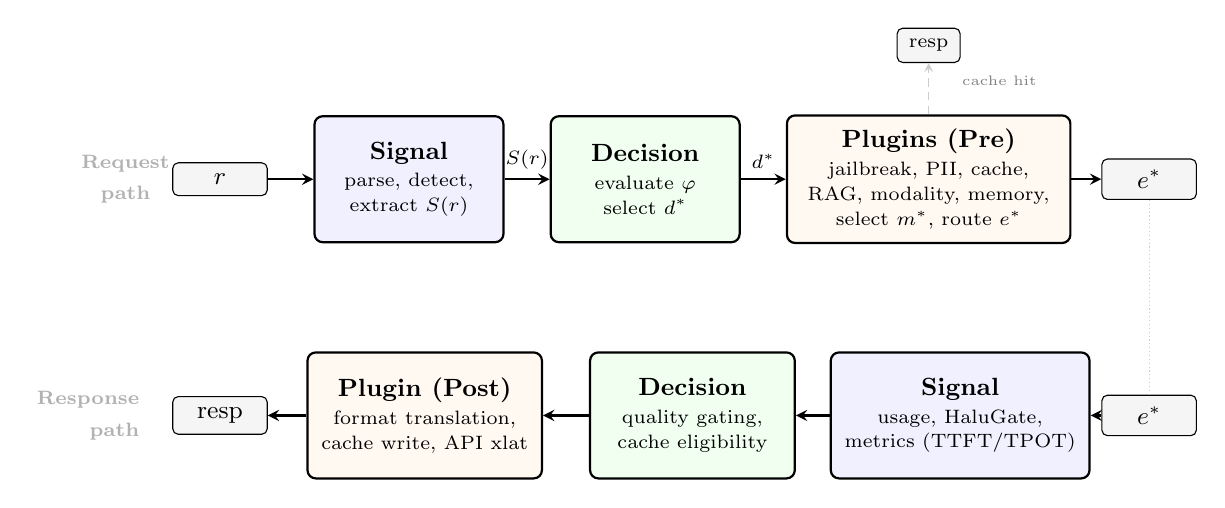
\begin{tikzpicture}[
    node distance=0.3cm,
    phase/.style={rectangle, draw, thick, rounded corners=3pt,
                  align=center, inner sep=5pt, font=\small,
                  minimum height=1.6cm},
    io/.style={rectangle, draw, rounded corners=2pt, fill=black!4,
               font=\small, inner sep=4pt, align=center,
               minimum width=1.2cm},
    sub/.style={font=\scriptsize, align=left, text=black!70},
    arr/.style={->, >=stealth, thick},
    darr/.style={->, >=stealth, densely dashed, gray!40},
    pathlbl/.style={font=\scriptsize\bfseries, text=gray!60},
  ]

  % ===== Request path (top, left → right) =====
  \node[pathlbl] at (-0.4, 1.6) {Request};
  \node[pathlbl] at (-0.4, 1.2) {path};

  \node[io] (req) at (0.8, 1.4) {$r$};

  % Layer 1: Signal
  \node[phase, fill=blue!6, minimum width=2.4cm] (sig) at (3.2, 1.4) {%
    \textbf{Signal}\\[-1pt]
    {\scriptsize parse, detect,}\\[-2pt]
    {\scriptsize extract $S(r)$}};

  % Layer 2: Decision
  \node[phase, fill=green!6, minimum width=2.4cm] (dec) at (6.2, 1.4) {%
    \textbf{Decision}\\[-1pt]
    {\scriptsize evaluate $\varphi$}\\[-2pt]
    {\scriptsize select $d^*$}};

  % Layer 3: Plugins (Pre) + Select + Route
  \node[phase, fill=orange!5, minimum width=3.6cm] (plug) at (9.8, 1.4) {%
    \textbf{Plugins (Pre)}\\[-1pt]
    {\scriptsize jailbreak, PII, cache,}\\[-2pt]
    {\scriptsize RAG, modality, memory,}\\[-2pt]
    {\scriptsize select $m^*$, route $e^*$}};

  \node[io] (ep) at (12.6, 1.4) {$e^*$};

  % Request arrows
  \draw[arr] (req) -- (sig);
  \draw[arr] (sig) -- node[above, font=\scriptsize]{$S(r)$} (dec);
  \draw[arr] (dec) -- node[above, font=\scriptsize]{$d^*$} (plug);
  \draw[arr] (plug) -- (ep);

  % Cache hit short-circuit
  \node[io, minimum width=0.8cm, font=\scriptsize] (hit) at (9.8, 3.1) {resp};
  \draw[darr] (plug.north) -- (hit.south);
  \node[font=\tiny, text=gray, anchor=west] at (10.1, 2.65) {cache hit};

  % ===== Response path (bottom, right → left) =====
  \node[pathlbl, anchor=east] at (-0.1, -1.4) {Response};
  \node[pathlbl, anchor=east] at (-0.1, -1.8) {path};

  \node[io] (ep2) at (12.6, -1.6) {$e^*$};

  % Layer 1: Signal (response) — first stage after e*
  \node[phase, fill=blue!6, minimum width=2.6cm] (rsig) at (10.2, -1.6) {%
    \textbf{Signal}\\[-1pt]
    {\scriptsize usage, HaluGate,}\\[-2pt]
    {\scriptsize metrics (TTFT/TPOT)}};

  % Layer 2: Decision (response)
  \node[phase, fill=green!6, minimum width=2.6cm] (rdec) at (6.8, -1.6) {%
    \textbf{Decision}\\[-1pt]
    {\scriptsize quality gating,}\\[-2pt]
    {\scriptsize cache eligibility}};

  % Layer 3: Plugins (Post)
  \node[phase, fill=orange!5, minimum width=2.6cm] (post) at (3.4, -1.6) {%
    \textbf{Plugin (Post)}\\[-1pt]
    {\scriptsize format translation,}\\[-2pt]
    {\scriptsize cache write, API xlat}};

  \node[io] (resp) at (0.8, -1.6) {resp};

  % Response arrows (right → left): Signal → Decision → Plugin
  \draw[arr] (ep2) -- (rsig);
  \draw[arr] (rsig) -- (rdec);
  \draw[arr] (rdec) -- (post);
  \draw[arr] (post) -- (resp);

  % Vertical connection: provider endpoint shared
  \draw[thin, densely dotted, gray!40] (ep.south) -- ++(0, -0.15) -| (ep2.north);

\end{tikzpicture}
\caption{Bidirectional request processing pipeline aligned with the three-layer architecture.  \textbf{Request path} (top, left$\to$right): the signal layer parses and extracts $S(r)$; the decision layer evaluates Boolean formulas to select $d^*$; the plugin chain executes pre-processing (safety, caching, RAG, memory), model selection, and endpoint routing.  A cache hit short-circuits the pipeline (dashed).  \textbf{Response path} (bottom, right$\to$left): the same three layers operate in the same order---the signal layer extracts response-side signals (token usage, HaluGate hallucination scores, streaming latency metrics); the decision layer evaluates quality gating and cache eligibility; plugins perform format translation, cache writes, and API translation.}
\label{fig:extproc_pipeline}
\end{figure}

The stages execute in strict order:
(1)~API translation (Responses API $\to$ Chat Completions if applicable, see \Cref{subsec:responses_api});
(2)~request parsing and provider detection;
(3)~signal extraction and decision evaluation (\Cref{sec:signal_engine,sec:decision_engine});
(4)~jailbreak detection (\Cref{sec:safety});
(5)~PII detection (\Cref{sec:safety});
(6)~semantic cache lookup (\Cref{sec:plugins})---cache hits terminate the pipeline with an immediate response;
(7)~RAG context injection (\Cref{sec:memory_rag});
(8)~modality routing (text vs.\ diffusion);
(9)~memory retrieval (\Cref{sec:memory_rag});
(10)~model selection (\Cref{sec:model_selection}), system prompt injection, and header mutation;
(11)~multi-endpoint resolution and provider-specific auth injection (\Cref{subsec:multi_endpoint,subsec:authz_factory}).

\subsection{Multi-Endpoint and Multi-Provider Routing}
\label{subsec:multi_endpoint}

Production deployments often span multiple model backends across different providers and geographic regions.
The system supports \emph{multi-endpoint routing} as a first-class concept:

\begin{definition}[Endpoint Topology]
An endpoint topology $\mathcal{E} = \{(e_i, w_i, p_i, \alpha_i)\}_{i=1}^{L}$ defines $L$ endpoints, each with a weight $w_i \in (0, 1]$ (normalized: $\sum_i w_i = 1$), a provider type $p_i \in \mathcal{P}$, and an auth profile $\alpha_i$.
\end{definition}

Once semantic model selection identifies a target model $m^*$, the endpoint router resolves $m^*$ to a concrete endpoint $e^*$ from the set of endpoints serving that model.
Weighted random selection with sticky session affinity distributes load proportionally.
Failover cascades to the next-weighted endpoint on backend errors.

Each endpoint may use a different provider (e.g., the same logical model ``gpt-4o'' served by both OpenAI and Azure OpenAI).
The system performs \emph{provider-specific protocol translation} transparently:

\begin{itemize}[leftmargin=*]
  \item \textbf{OpenAI / Azure OpenAI}: Native Chat Completions and Responses API formats.
  \item \textbf{Anthropic}: Translation between OpenAI message schema and Anthropic Messages API (system prompt handling, tool use mapping).
  \item \textbf{Bedrock / Vertex AI}: Cloud-provider-specific request wrapping, authentication (SigV4 for AWS, OAuth for GCP), and response unwrapping.
  \item \textbf{Gemini}: Conversion between OpenAI function-calling schema and Gemini tool declarations.
  \item \textbf{vLLM / Local}: Direct OpenAI-compatible passthrough to self-hosted vLLM instances.
\end{itemize}

This abstraction allows routing decisions to reference models by capability (``best coding model'') rather than by provider-specific endpoint, and allows the same decision configuration to operate across different deployment topologies.

\subsection{OpenAI Responses API Support}
\label{subsec:responses_api}

The system provides full support for the OpenAI Responses API, which extends Chat Completions with stateful multi-turn conversation management.

The Responses API introduces \texttt{previous\_response\_id} chaining: each response carries a unique identifier, and subsequent requests can reference it to maintain conversation context without the client retransmitting the full message history.
The routing system handles this by:

\begin{enumerate}[leftmargin=*]
  \item \textbf{Inbound translation}: Responses API requests (with \texttt{input} field and \texttt{previous\_response\_id}) are normalized to Chat Completions format for signal extraction and decision evaluation, which operate on the unified internal representation.
  \item \textbf{State management}: Conversation history is stored in the persistent memory layer (\Cref{sec:memory_rag}), keyed by response ID, enabling context retrieval across turns.
  \item \textbf{Outbound translation}: Chat Completions responses from backends are wrapped in Responses API format (with \texttt{id}, \texttt{output} array, \texttt{usage} breakdown) before returning to the client.
  \item \textbf{Routing consistency}: The decision engine can optionally pin conversation turns to the same model to avoid mid-conversation quality shifts.
\end{enumerate}

This translation layer is transparent to both the signal engine and the downstream model backends, enabling all routing, safety, and caching features to operate identically on Responses API and Chat Completions traffic.

\subsection{Authorization Factory}
\label{subsec:authz_factory}

Multi-provider deployments require diverse authentication mechanisms.
The system implements a \emph{pluggable authorization factory} that abstracts auth concerns from routing logic:

\begin{definition}[Auth Provider]
An auth provider $\alpha: (\text{Request}, \text{Endpoint}) \to \text{Headers}'$ is a function that enriches outbound request headers with provider-appropriate credentials.
\end{definition}

The factory supports multiple auth provider types:

\begin{itemize}[leftmargin=*]
  \item \textbf{API Key}: Static bearer tokens or API keys, optionally per-endpoint, with header name customization (e.g., \texttt{Authorization}, \texttt{x-api-key}, \texttt{api-key}).
  \item \textbf{OAuth2 / OIDC}: Token acquisition with automatic refresh, supporting client credentials and authorization code flows.
  \item \textbf{Cloud IAM}: AWS SigV4 signing for Bedrock, Google service account tokens for Vertex AI, Azure AD tokens for Azure OpenAI.
  \item \textbf{Passthrough}: Forwarding the client's original credentials to the backend, used for deployments where the client authenticates directly.
  \item \textbf{Custom}: User-defined auth plugins registered at startup, enabling integration with enterprise identity providers (LDAP, SAML, custom JWT issuers).
\end{itemize}

The auth factory is invoked \emph{after} decision evaluation and model selection, injecting provider-specific credentials into the outbound request headers.
This separation ensures that routing decisions are auth-agnostic: the decision engine selects models based on capability and cost, and the auth layer handles the mechanics of reaching each provider's endpoint.

The \texttt{authz} signal type in the signal engine (\Cref{sec:signal_engine}) is complementary but distinct: it performs \emph{inbound} authorization (verifying that the requesting user or API key has permission to access specific models or decisions), while the auth factory handles \emph{outbound} authentication (proving the router's identity to backend providers).

\subsection{Response Body Pipeline}

The response path performs:
(1)~token usage extraction for cost accounting;
(2)~format translation (provider-specific $\to$ OpenAI format);
(3)~streaming metrics computation (TTFT, TPOT);
(4)~hallucination detection via HaluGate (\Cref{sec:halugate});
(5)~semantic cache writes for cache misses;
(6)~Responses API translation (Chat Completions $\to$ Responses API format, if applicable).

\subsection{Concurrency Model}

Each gRPC stream (one per HTTP request) runs in an independent goroutine, processing its four phases sequentially.
Within a request, signal extraction launches parallel coroutines for independent classifiers.
Shared state (classifier models, cache backends, configuration, auth token caches) is read concurrently by all active streams, with synchronization limited to cache writes, auth token refreshes, and metric updates.
